\subsubsection{24.12.2015}
\textit{\textbf{Time frame:}} 17:00-22:00 

The elevator was tested while the robot was standing on the horisontal surface (figure \ref{Elevator2.5}). It worked ok. The full extraction took 4.5 seconds.

The length of cables on the elevator were adjusted so as make the same tension on both of them. It will help to avoid the bend of the elevator while extracting.

\begin{figure}[H]
	\begin{minipage}[h]{1\linewidth}
		\center{\includegraphics[scale=0.2]{3Engineering/5Team_meetings/days_of_meetings/2015.12.24/images/01}}
		\caption{Testing of the elevator}
		\label{Elevator2.5}
	\end{minipage}
\end{figure}

The wiring to the top section of the elevator (to the bucket and mechanism for shifting the bucket) was held (figure \ref{Wiring1.3}, \ref{Controllers1.4}).

\begin{figure}[H]
	\begin{minipage}[h]{0.47\linewidth}
		\center{\includegraphics[scale=0.2]{3Engineering/5Team_meetings/days_of_meetings/2015.12.24/images/02}}
		\caption{Wiring to the bucket}
		\label{Wiring1.3}
	\end{minipage}
	\hfill
	\begin{minipage}[h]{0.47\linewidth}
		\center{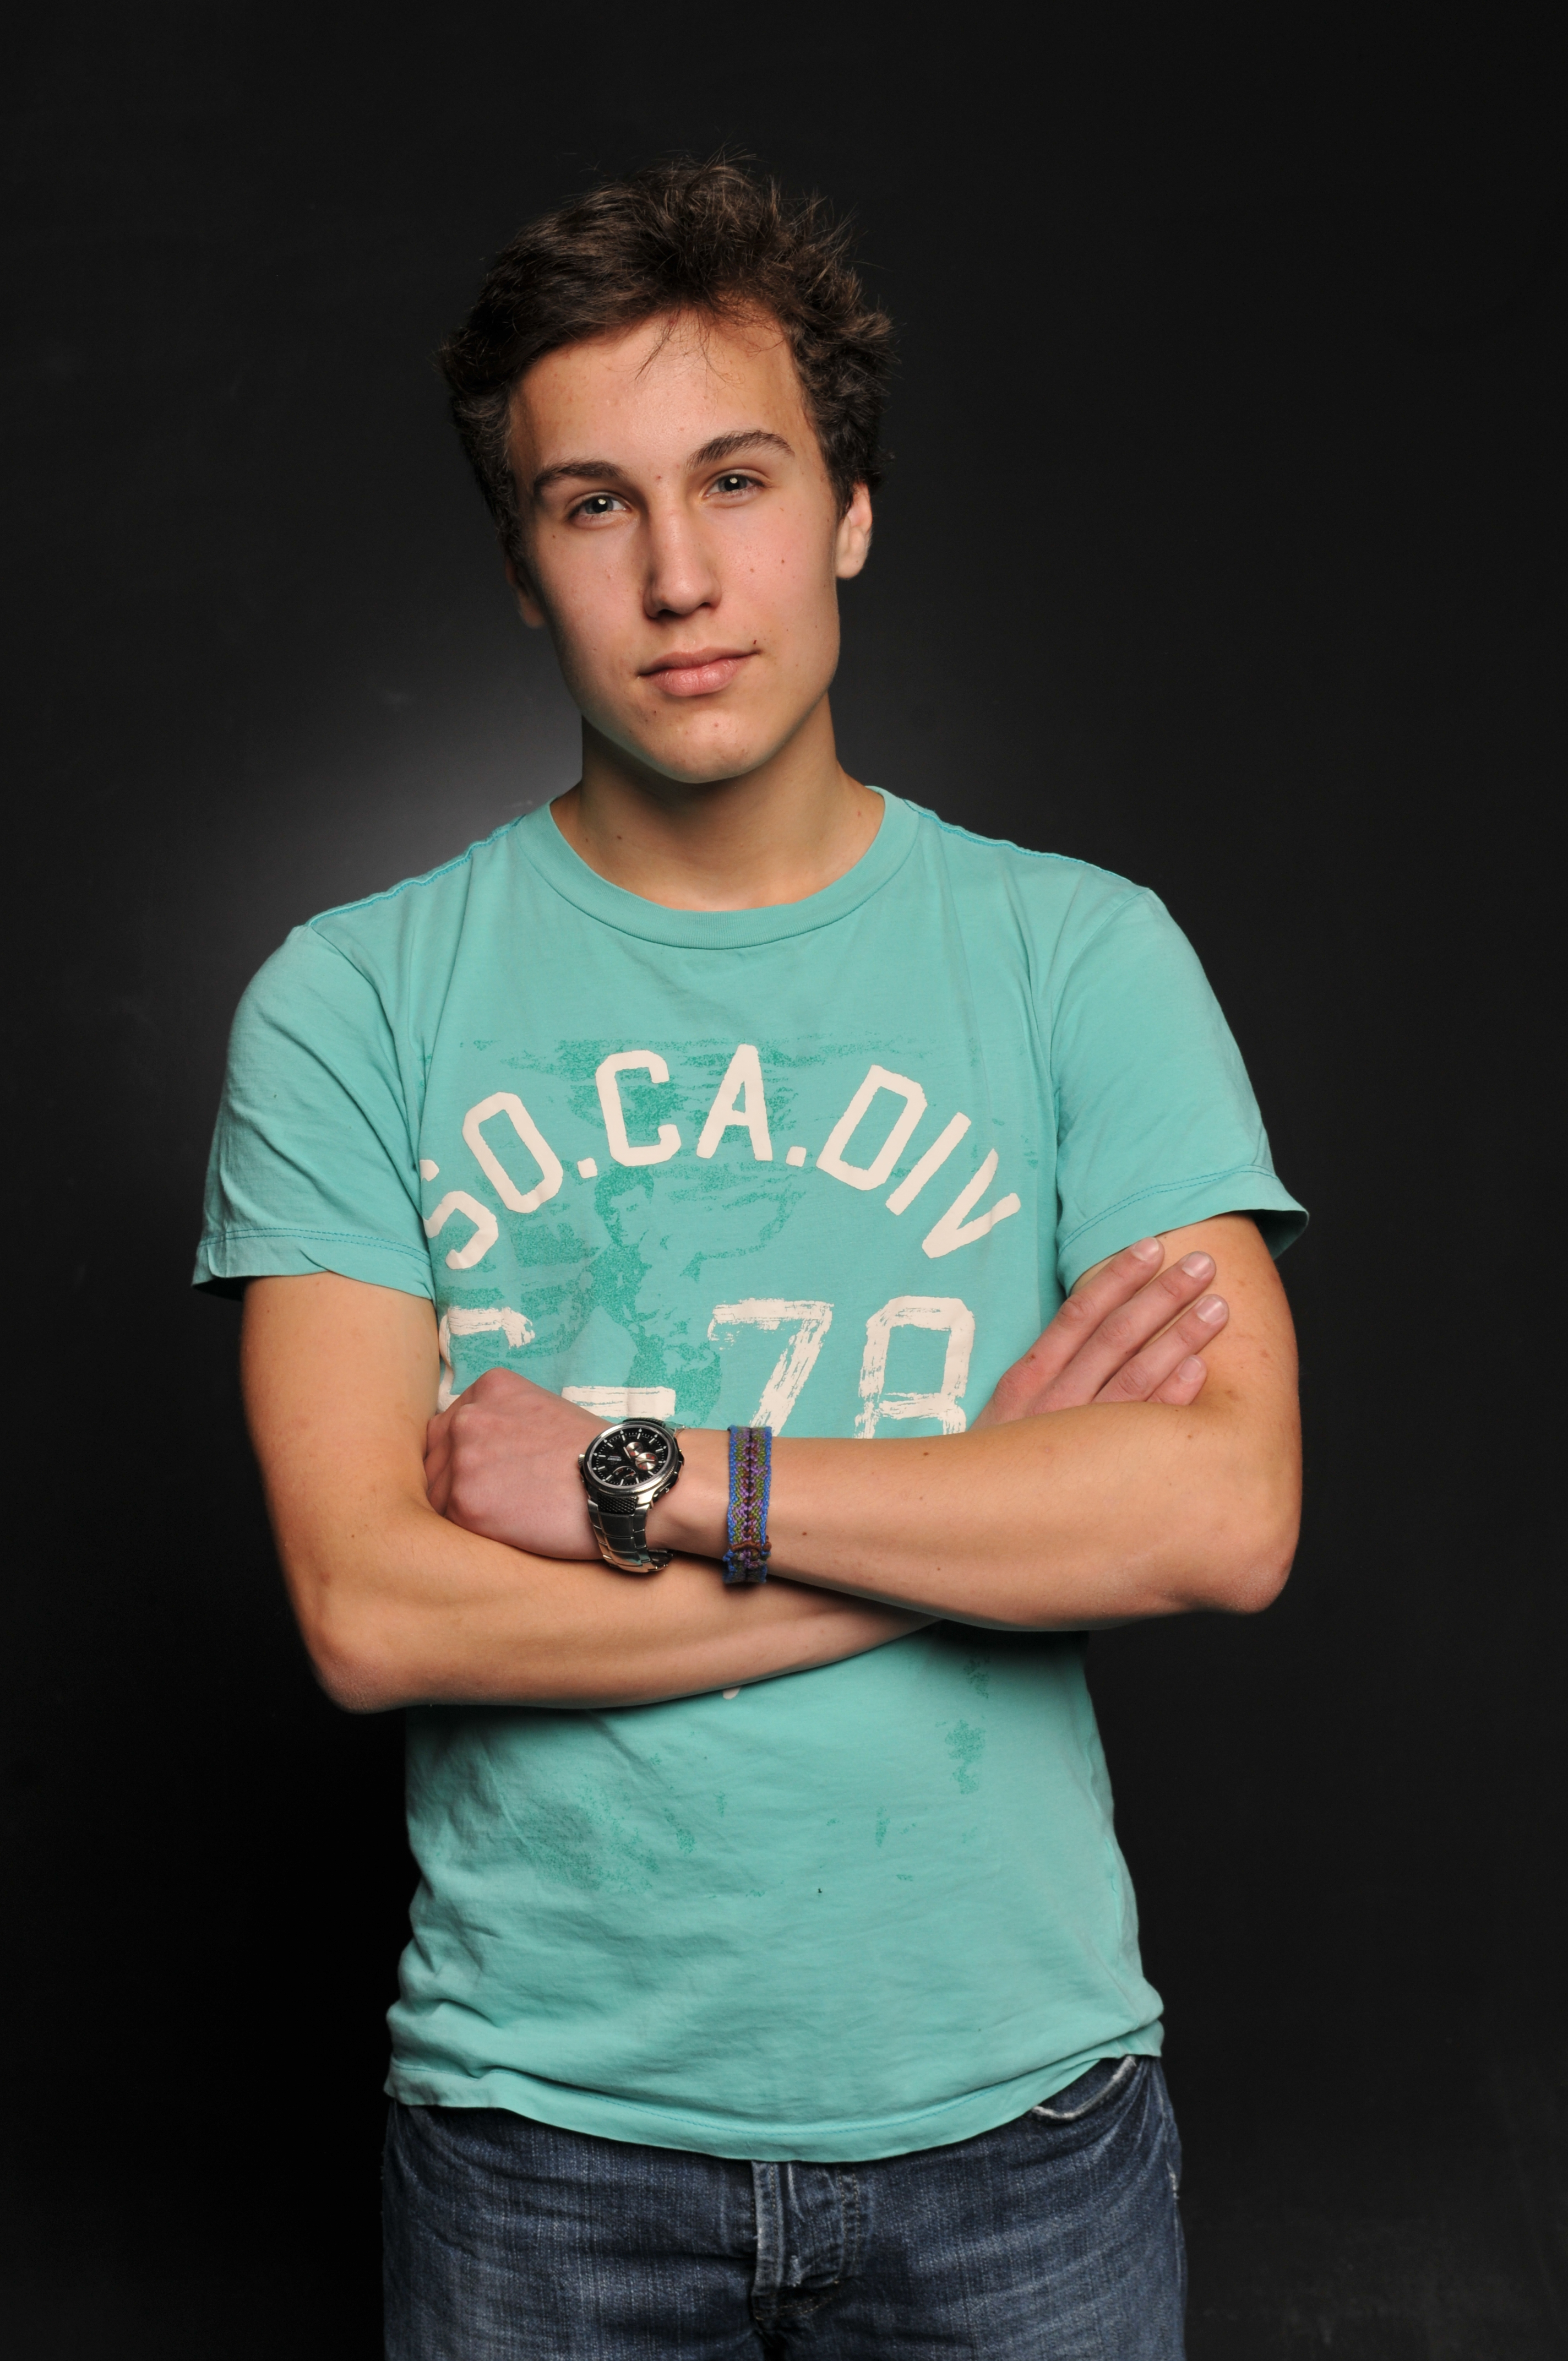
\includegraphics[scale=0.2]{3Engineering/5Team_meetings/days_of_meetings/2015.12.24/images/03}}
		\caption{The servo controller}
		\label{Controllers1.4}
	\end{minipage}
\end{figure}

It was investigated that the beams at the sides, to which the blocks attached, are narrowing because of the tension forse of the cable. To prevent this bending of beams there was installed another beam between them (figure \ref{Winch2.8}).

There were also installed shores for cables that will prevent them from tangling (only for one cable this day).

\begin{figure}[H]
	\begin{minipage}[h]{1\linewidth}
		\center{\includegraphics[scale=0.2]{3Engineering/5Team_meetings/days_of_meetings/2015.12.24/images/04}}
		\caption{Beam with shores (the current image was taken after all the shores were installed)}
		\label{Winch2.8}
	\end{minipage}
\end{figure}
